% =====================================================================
%  The Radiomics--Microbiome Axis Layer
%  Manuscript-style paper (two-column article, zero external .cls dep).
%  Restructured 2026-05-18 from the single-column proposal report,
%  which is preserved unmodified at:
%     docs/paper/proposal/report_sanomap_radiomics_layer.tex
%  Build:  pdflatex paper_sanomap_radiomics_layer.tex   (run twice)
% =====================================================================
\documentclass[10pt,twocolumn,letterpaper]{article}

\usepackage[utf8]{inputenc}
\usepackage[T1]{fontenc}
\usepackage{geometry}
\geometry{margin=0.75in, columnsep=0.28in}
\usepackage{titlesec}
\usepackage{enumitem}
\usepackage{booktabs}
\usepackage{amsmath}
\usepackage{amssymb}
\usepackage{tikz}
\usetikzlibrary{positioning,arrows.meta,fit,backgrounds,calc}
\usepackage[hidelinks]{hyperref}
% microtype intentionally omitted: basictex Type1 fonts are non-scalable,
% so pdftex font expansion is fatal. Reliability > typographic polish here.

% Compact list spacing for a dense two-column manuscript
\setlist{nosep,leftmargin=1.2em}

% Journal-style section headings
\titleformat{\section}
  {\normalfont\large\bfseries}{\thesection.}{0.5em}{}
\titleformat{\subsection}
  {\normalfont\normalsize\bfseries}{\thesubsection}{0.5em}{}
\titlespacing*{\section}{0pt}{1.4ex plus 0.4ex}{0.8ex}
\titlespacing*{\subsection}{0pt}{1.1ex plus 0.3ex}{0.6ex}

\setlength{\parindent}{1em}
\setlength{\parskip}{0.15ex}

\title{\vspace{-3ex}\textbf{The Radiomics--Microbiome Axis Layer:\\
A Hybrid Text--Vision Pipeline with Five-Gate\\
Acceptance for Knowledge-Graph Extension}}

\author{Junseong Lee\\
\small SanoMap Project --- Radiomics-Microbiome Axis Layer\\
\small \texttt{junseong.lee652@gmail.com}}

\date{\small Draft of \today\ \textbf{(pre-print; benchmark metrics gated, see \S\ref{sec:eval})}}

\begin{document}

\twocolumn[
\begin{@twocolumnfalse}
\maketitle
\begin{abstract}
\noindent
Literature-mined microbiome knowledge graphs such as the SanoMap MINERVA
platform connect microbes directly to diseases but omit the quantitative,
tissue-level imaging phenotypes that mechanistically link them, and much
of the quantitative microbe--imaging correlation evidence is additionally
locked inside figures, invisible to text-only pipelines. We build a
radiomics-first intermediary layer that inserts \texttt{RadiomicFeature}
and \texttt{BodyCompositionFeature} nodes between microbe and disease. A
two-track pipeline---a text track over 1{,}016 open-access papers and a
vision track that reads correlation heatmaps with a vision-language
model---feeds a five-gate acceptance model: dense-retrieval candidate
generation, UMLS type-grounded entity sanitization with a species-specific
NER head (LINNAEUS F1$=$0.9649), self-consistency relation acceptance,
dual-verifier vision consensus behind a deterministic pre-verifier gate
chain (caption, colorbar-detect, range-sanity, sign-check), and a
stratified gold-label benchmark. Accepted edges are reconciled into a
single provenance-stamped graph export and loaded into Neo4j with a
read-only query layer. The graph carries 74 phenotype--disease
\texttt{ASSOCIATED\_WITH} edges, 29 signed microbe--disease edges, and---after
a retroactive vision audit and a graph reconciliation that composed both
the vision retraction and the UMLS drop onto one base---7
\texttt{CORRELATES\_WITH} microbe--feature edges (1 vision, 6 text),
closing 62 traversable
microbe$\rightarrow$feature$\rightarrow$disease paths that a single-hop
schema cannot express. The vision track's measured contribution is
deliberately scoped to one audited case-study figure plus a
hallucination-resistant gating methodology. Precision, recall and
intra-annotator Cohen's $\kappa$ are gated on a non-negotiable 14-day
temporal re-labeling window and are reported as pending rather than
estimated. Making the imaging phenotype explicit is feasible, reviewable,
and reproducible; the engineering contribution is the acceptance-gate
architecture and an honest accounting of where each evidence modality
does and does not deliver.

\vspace{1ex}
\noindent\textbf{Keywords:} knowledge graph; radiomics; gut microbiome;
vision-language models; biomedical relation extraction; Neo4j; evidence
provenance.
\end{abstract}
\vspace{3ex}
\end{@twocolumnfalse}
]

% =====================================================================
\section{Introduction}
% =====================================================================

Biomedical knowledge graphs derive their clinical value from the
completeness of the evidence they encode. A lineage of curated
microbe--disease databases---HMDAD~\cite{ma2016hmdad},
gutMDisorder~\cite{qi2022gutmdisorder}, GMMAD~\cite{wang2023gmmad},
Amadis~\cite{li2021amadis}, Disbiome~\cite{janssens2018disbiome},
MDIDB~\cite{wu2021mdidb}---established the value of structuring scattered
literature into queryable graphs, but their reliance on manual curation
caps scalability. Transformer-based language models and generative AI now
enable large-scale automation of this construction~\cite{devlin2019bert,beltagy2019scibert,karkera2023microbe,wenhao2022markergenie};
hallucination remains the dominant residual risk in clinical
deployment~\cite{aurangzeb2023hallucinations}. The SanoMap project's
MINERVA platform (Microbiomes Network Research and Visualization
Atlas)~\cite{langarica2025minerva} demonstrates the
LLM-grounded-on-literature approach at scale: it processes 129{,}719
publications into 66{,}400 microbe--disease relationships, producing a
clinically navigable graph that surpasses every prior curated baseline on
both coverage and provenance traceability.

Yet MINERVA's graph encodes a structurally incomplete picture by design: it
connects microbes directly to diseases but omits the quantitative,
tissue-level intermediate phenotypes that explain the biological mechanism
linking them~\cite{langarica2025minerva}.
Radiomics~\cite{lambin2012,aerts2014} and body-composition
imaging~\cite{cruzjentoft2019ewgsop2} provide exactly these intermediaries.
Skeletal muscle index, visceral adipose tissue fraction, liver fat fraction,
and GLCM texture signatures are extracted directly from CT and MRI and are
established biomarkers for sarcopenia, nonalcoholic fatty liver
disease~\cite{tilg2022gutliver}, and colorectal cancer. The literature
increasingly demonstrates that gut microbiome composition measurably
influences these specific tissue-level phenotypes~\cite{ticinesi2019gutmuscle,cani2008endotoxemia,botticelli2023qta}---making
them natural intermediary nodes in any complete microbiome--disease graph.

A second structural gap concerns the evidence modality itself. Text-mining
pipelines extract findings authors highlight in prose, but much of the
quantitative correlation data linking microbial taxa to imaging feature
values is encoded in figures. Gradient correlation heatmaps display matrices
of $r$-values linking dozens of taxa to radiomic measurements---data NLP
alone cannot parse. This is a systematic evidence loss in text-only
pipelines.

This work addresses both gaps. The central research questions are:
\textbf{(RQ1)} Can a hybrid pipeline combining large language models and
vision-language models, with deterministic verification, reliably extract
quantitative correlation coefficients directly from medical figures? And
\textbf{(RQ2)} does adding radiomics as an ontological layer---filling the
microbe$\rightarrow$imaging-phenotype$\rightarrow$disease path---meaningfully
increase the clinical completeness of the MINERVA knowledge graph? A third,
engineering question runs underneath both: \textbf{(RQ3)} what acceptance
architecture keeps such a hybrid graph \emph{reviewable}---auditable
edge-by-edge---rather than merely large?

This paper's contribution is not a claim of upstream parity. It is (i) an
explicit intermediary-layer ontology, (ii) a five-gate acceptance model that
converts a proof-of-concept pipeline into a measurable artifact, (iii) a
retroactive audit that honestly rescopes the vision track after a structural
verifier weakness was found, and (iv) a single reconciled, provenance-stamped
graph reproducibly loadable into Neo4j.

% =====================================================================
\section{The Intermediary Layer: Concept and Schema}
% =====================================================================

\subsection{Core idea}

MINERVA's current graph encodes
\texttt{(Microbe)$\rightarrow$[ASSOCIATED\_WITH]$\rightarrow$(Disease)}. This
edge is clinically underspecified. The biologically accurate path is

\begin{center}
\small
\texttt{Microbe} $\rightarrow$ \textit{correlates with} $\rightarrow$
\texttt{Radiomic/BodyComp\-Feature} $\rightarrow$ \textit{associates with}
$\rightarrow$ \texttt{Disease}.
\end{center}

This three-node path is documented concretely: \textit{Prevotella
nigrescens} correlates with GLCM Correlation texture on CT at $r=0.95$
(PMC10605408; PMID~37894458~\cite{botticelli2023qta}); cirrhosis dysbiosis
enriches Proteobacteria alongside measurable changes in liver surface
nodularity and visceral fat~\cite{tilg2022gutliver};
\textit{Bifidobacterium} depletion co-occurs with elevated visceral
adipose tissue and downstream obesity~\cite{cani2008endotoxemia}. These are quantitatively measured, directly
evidenced relations that a text-only microbe$\rightarrow$disease edge
collapses into a single mechanism-blind link. Making the intermediary
explicit enables queries impossible in MINERVA's schema, e.g.\ ``what CT
texture signature mediates the association between gut dysbiosis and
sarcopenia?''

\begin{figure*}[t]
\centering
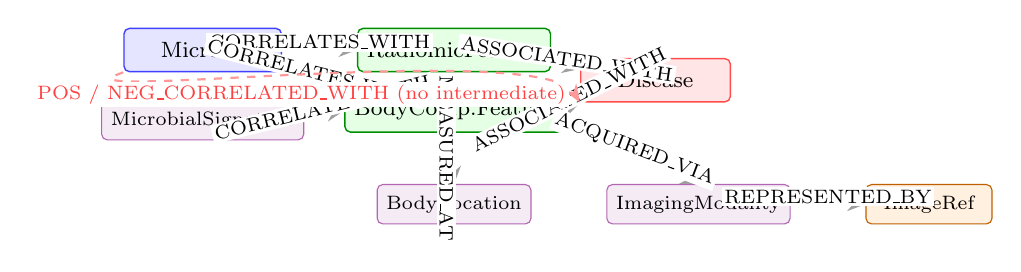
\begin{tikzpicture}[
  >=Stealth,
  node distance=0.55cm and 0.95cm,
  every node/.style={font=\footnotesize, align=center},
  micr/.style={draw=blue!75, fill=blue!10, rounded corners=2pt, minimum width=2.0cm, minimum height=0.55cm, line width=0.5pt},
  feat/.style={draw=green!55!black, fill=green!10, rounded corners=2pt, minimum width=2.4cm, minimum height=0.55cm, line width=0.5pt},
  dis/.style={draw=red!70, fill=red!10, rounded corners=2pt, minimum width=1.9cm, minimum height=0.55cm, line width=0.5pt},
  back/.style={draw=violet!60, fill=violet!8, rounded corners=2pt, minimum width=1.8cm, minimum height=0.5cm, font=\scriptsize, line width=0.4pt},
  img/.style={draw=orange!75!black, fill=orange!12, rounded corners=2pt, minimum width=1.6cm, minimum height=0.5cm, font=\scriptsize, line width=0.4pt},
  e/.style={->, thick, draw=gray!75},
  el/.style={font=\scriptsize, midway, sloped, above=-1pt, fill=white, inner sep=1pt}
]
\node[micr] (M) {Microbe};
\node[feat, right=of M] (RF) {RadiomicFeature};
\node[feat, below=0.2cm of RF] (BCF) {BodyComp.Feature};
\node[dis, right=of $(RF)!0.5!(BCF)$, xshift=0.65cm] (D) {Disease};
\node[back, below=0.35cm of M, xshift=-0.0cm] (MS) {MicrobialSignature};
\node[back, below=0.65cm of BCF] (BL) {BodyLocation};
\node[back, right=of BL] (IM) {ImagingModality};
\node[img, right=of IM] (IR) {ImageRef};

\draw[e] (M) -- node[el]{CORRELATES\_WITH} (RF);
\draw[e] (M.south east) -- node[el]{CORRELATES\_WITH} (BCF.north west);
\draw[e] (MS.east) -- node[el]{CORRELATES\_WITH} (BCF.west);
\draw[e] (RF) -- node[el]{ASSOCIATED\_WITH} (D);
\draw[e] (BCF.east) -- node[el]{ASSOCIATED\_WITH} (D.south west);
\draw[e] (BCF.south) -- node[el,below=-1pt]{MEASURED\_AT} (BL.north);
\draw[e] (BCF.south east) -- node[el]{ACQUIRED\_VIA} (IM.north);
\draw[e] (IM) -- node[el]{REPRESENTED\_BY} (IR);
\draw[e, dashed, draw=red!40] (M.south west) ..controls +(-1.2,-0.4) and +(-0.5,0.8).. node[el, sloped=false, below=2pt]{\textcolor{red!75}{POS / NEG\_CORRELATED\_WITH (no intermediate)}} (D.south west);
\end{tikzpicture}
\caption{The Imaging-Phenotype Layer ontology. Solid arrows: evidence-typed
edges promoted to the graph (precision pole \texttt{RadiomicFeature} +
coverage pole \texttt{BodyCompositionFeature}). Dashed red arrow: the
upstream MINERVA \texttt{POSITIVELY\_/NEGATIVELY\_CORRELATED\_WITH} edge that
\emph{collapses} the imaging-phenotype intermediary into a single
mechanism-blind link. The intermediate layer makes the biology auditable
edge-by-edge; the dashed shortcut is retained for backward compatibility but
does not substitute for the three-hop traversal.}
\label{fig:schema}
\end{figure*}

\subsection{Node and edge ontology}

Node types extend MINERVA: \texttt{RadiomicFeature} (texture, morphological,
intensity features---GLCM, wavelet, first-order, shape---IBSI-aligned
naming~\cite{zwanenburg2020ibsi,vanGriethuysen2017pyradiomics});
\texttt{BodyCompositionFeature} (sarcopenia, visceral adipose tissue,
skeletal muscle index, liver fat fraction, myosteatosis---clinical aggregate
quantitative imaging biomarkers, dominant in microbe$\rightarrow$imaging
literature~\cite{ticinesi2019gutmuscle,cruzjentoft2019ewgsop2});
\texttt{BodyLocation}; \texttt{ImagingModality}; \texttt{ImageRef} (verified
figure references with Vision Track provenance); \texttt{Microbe} /
\texttt{MicrobialSignature}; and \texttt{Disease}.
Figure~\ref{fig:schema} summarizes the schema.

The direct-evidence edge policy is deliberately evidence-typed:
quantitatively verified microbe$\rightarrow$feature edges (a vision-confirmed
$r$-value) use \texttt{CORRELATES\_WITH}; text co-mention
feature$\rightarrow$disease edges use \texttt{ASSOCIATED\_WITH}; signed
microbe$\rightarrow$disease edges use
\texttt{POSITIVELY\_/NEGATIVELY\_CORRELATED\_WITH}; structural edges use
\texttt{MEASURED\_AT}, \texttt{ACQUIRED\_VIA}, \texttt{REPRESENTED\_BY}. The
\texttt{CORRELATES\_WITH}/\texttt{ASSOCIATED\_WITH} distinction preserves
evidence-level semantics across the graph and is never collapsed. Within-paper
bridge matches that only share disease context are written to an audit
artifact as hypotheses and are \emph{never} ingested as asserted edges.

% =====================================================================
\section{Methods}
% =====================================================================

\subsection{Data sourcing}

Data was sourced from PubMed Central Open Access via a multi-lane query
strategy over six clinical domains where the microbiome--radiomics link is
best evidenced: (1) strict radiomics + microbiome; (2) body composition +
microbiome; (3) liver radiomics + microbiome; (4) bone-density (DXA) +
microbiome; (5) lung-CT phenotypes + microbiome; (6) colorectal imaging +
microbiome. The corpus spans \textbf{1{,}016 papers} (640 from the initial
three lanes plus 376 net-new from lanes 4--6), with open-access full text
retrieved where a PMCID exists. Review, meta-analysis, and protocol papers
are excluded as non-direct-evidence targets.

\subsection{Two-track pipeline}

The \textbf{Text Track} extracts phenotype--disease associations at scale. A
vocabulary-matched stage maps imaging-phenotype terminology to canonical
names; microbial NER uses \texttt{d4data/biomedical-ner-all} on Apple Silicon
MPS, disease NER uses the \texttt{en\_ner\_bc5cdr\_md} spaCy
pipeline~\cite{neumann2019scispacy,li2016bc5cdr}; a shared span-cleanup
layer rejects wordpiece artifacts, generic placeholders, and clause-prefix
fragments before relation classification.

The \textbf{Vision Track} addresses the figure-data gap. A vision-language
model proposes $r$-values for microbe$\rightarrow$feature correlations read
from heatmap figures; each proposal is deterministically cross-checked
against the figure's gradient color-scale legend at pixel level.

\subsection{Five-gate acceptance model}
\label{sec:gates}

Tracks alone do not establish research-defensibility; structurally distinct
gates do. A candidate edge enters the graph only when every gate that applies
to its evidence track passes.

\begin{enumerate}
\item \textbf{Retrieval (text).} A dense-retrieval index over
\texttt{BioClinical-ModernBERT-base} embeddings (mean-pooled, L2-normalized;
FAISS~\cite{johnson2019faiss} where available, NumPy cosine fallback at
$\sim$30k sentences) replaces the original hand-curated 25-alias substring
filter, removing its recall ceiling on paraphrastic mentions (``loss of
muscle mass at L3''). Per-feature similarity threshold $\tau$ is calibrated
per concept against labeled data.

\item \textbf{Entity sanitization (UMLS TUI grounding).} Microbial surface
forms must ground to a microbe-class UMLS~\cite{bodenreider2004umls}
Semantic Type at similarity $\geq 0.85$; accept set $\{$T005 Virus, T007
Bacterium, T194 Archaeon, T204 Eukaryote$\}$ with an explicit non-microbe
model-organism deny-list. A live
audit of the 8 accepted text-derived microbe$\rightarrow$feature edges drops
25\% (2/8): the entity-type error \texttt{gut bacterial ClpB-like gene
function} (similarity 0.799 $<$ 0.85, grounded to ``Bacteria'' T007) and the
typo \texttt{bacteriodetes} (no UMLS match). The 25\% drop sits below the
30\% recalibration threshold; the 0.85 floor is retained.

\item \textbf{Relation acceptance (text).} Gemini 2.5 Flash-Lite,
7-sample temperature-varied self-consistency~\cite{wang2023selfconsistency},
full agreement required; measured full-consistency rate on the expanded
corpus is 0.916.

\item \textbf{Verification (vision) --- dual verifier behind a
pre-verifier gate chain.} See \S\ref{sec:visionaudit}; this gate's design is
itself a contribution.

\item \textbf{Evaluation (gold benchmark).} A 5-stratum sampler
(\texttt{accepted\_edge}, \texttt{gemini\_rejected}, \texttt{vocab\_excluded},
\texttt{recall\_probe}, \texttt{random\_co\_occurrence}) drawn deterministically
from the production candidate space yields a 66-row gold set. The schema
defines a 6-class primary label, three secondary labels, eight numbered
edge-case decisions, and a 14-day intra-annotator temporal-relabeling
protocol with Cohen's $\kappa \geq 0.80$ (binary collapse)
acceptance~\cite{landis1977kappa}.
Pass-1 used computer-aided manual annotation (LLM proposer, single human
reviewer who overrode 7 rows under an imaging-derived scope rule); Pass-2 is
the annotator's independent re-label after the temporal window. Metrics that
depend on Pass-1+Pass-2 are pending (\S\ref{sec:eval}).
\end{enumerate}

\subsection{Graph integration and reproducibility}
\label{sec:neo4j}

Earlier iterations emitted several divergent CSV vintages and a hand-runnable
Cypher script, with no single coherent ``current graph.'' This release adds a
deterministic reconciliation step: one command reads the authoritative
assembled artifacts, applies the documented post-audit drop-list (the
retracted Firmicutes vision edge; the two UMLS-failed
microbe$\rightarrow$feature edges), and emits a single
\texttt{graph\_export/} bundle---\texttt{nodes.csv},
\texttt{relationships.csv}, an idempotent \texttt{import.cypher}, and a
\texttt{manifest.json} recording source-artifact vintages, the git commit,
pre/post counts, and every drop with its reason. This step immediately earned
its keep: it found that the pre-existing prose headline (``8
\texttt{CORRELATES\_WITH}: 1 vision + 7 text'') had applied only the vision
retraction to the 9-edge superset and never composed in the separately
recorded UMLS drop; composing both onto one base yields the coherent 7 (1
vision + 6 text). The bundle loads into Neo4j through a thin driver loader; a
read-only query module exposes the canonical traversals (three-hop microbe$\rightarrow$feature$\rightarrow$disease;
feature-by-disease; signed microbe--disease; feature-by-location; full
modality-backbone chain; vision-verified edges). Provenance, not just the
graph, is the deliverable: every edge resolves back to a PMID, sentence, or
figure panel, and every count in this paper is reproducible from the
manifest.

% =====================================================================
\section{Results}
\label{sec:results}
% =====================================================================

\subsection{Extracted graph}

Across the 1{,}016-paper corpus the pipeline produced:

\begin{itemize}
\item \textbf{5{,}721} phenotype text mentions across 30 clinically
meaningful disease targets (initial 640-paper corpus; expanded-corpus
re-extraction in progress);
\item \textbf{74} \texttt{ASSOCIATED\_WITH} phenotype$\rightarrow$disease
edges (Gemini full-consistency 0.916 on the expanded corpus);
\item \textbf{29} signed microbe--disease edges (14 positive, 15 negative)
spanning cirrhosis, NAFLD, colorectal cancer, IBD, celiac disease, chronic
HCV, and SSc-associated pulmonary fibrosis;
\item \textbf{7} \texttt{CORRELATES\_WITH} microbe$\rightarrow$feature edges
\emph{after} reconciliation (\S\ref{sec:visionaudit}): 1 vision
(\textit{Prevotella nigrescens} $\rightarrow$ GLCM\_Correlation, $r=0.95$,
PMC10605408\_g004; pixel distance 0.05, support fraction 1.0) and 6 text
(Gemini 7/7);
\item \textbf{18} \texttt{BodyLocation} and \textbf{5}
\texttt{ImagingModality} nodes;
\item \textbf{189} reconciled relationship rows over \textbf{99} nodes. The
pre-reconciliation export reported 191 rows / 9 \texttt{CORRELATES\_WITH}; the
reconciliation step (\S\ref{sec:neo4j}) drops exactly two edges---one vision
retraction, one UMLS-failed entity---each recorded in the manifest with its
cited source artifact, rather than silently changing the headline.
\end{itemize}

Three surviving \texttt{CORRELATES\_WITH} edges close end-to-end three-hop
paths through features that also carry downstream \texttt{ASSOCIATED\_WITH}
disease edges---\textit{Ruminococcus}$\rightarrow$sarcopenia (37 diseases),
\textit{Peptostreptococcus stomatis}$\rightarrow$skeletal\_muscle\_index
(7)~\cite{ticinesi2019gutmuscle},
\textit{Eubacterium}$\rightarrow$visceral\_adipose\_tissue
(18)~\cite{cani2008endotoxemia}---yielding \textbf{62 traversable
microbe$\rightarrow$feature$\rightarrow$disease paths}, the query pattern
MINERVA's single-hop schema cannot express. This is direct evidence for
RQ2: the intermediary layer adds traversable mechanism, not just nodes.

\begin{table}[t]
\centering
\small
\caption{Reconciled graph metrics, post-audit (manifest of record:
\texttt{artifacts/graph\_export/manifest.json}). Counts compose the
2026-05-07 vision retraction and the UMLS entity-gate drop onto a single
189-row base.}
\label{tab:graphmetrics}
\begin{tabular}{@{}p{0.62\columnwidth}r@{}}
\toprule
\textbf{Metric} & \textbf{Value} \\
\midrule
Papers in corpus (PubMed Central OA, multi-lane) & 1{,}016 \\
Phenotype text mentions (initial 640-paper corpus) & 5{,}721 \\
Total reconciled relationship rows                & 189 \\
Total nodes (all labels)                          & 99 \\
\hspace{0.6em}\texttt{Microbe} nodes              & 23 \\
\hspace{0.6em}\texttt{Disease} nodes              & 38 \\
\hspace{0.6em}\texttt{RadiomicFeature} nodes      & 6 \\
\hspace{0.6em}\texttt{BodyCompositionFeature} nodes & 8 \\
\hspace{0.6em}\texttt{BodyLocation} nodes         & 18 \\
\hspace{0.6em}\texttt{ImagingModality} nodes      & 5 \\
\hspace{0.6em}\texttt{ImageRef} nodes             & 1 \\
\midrule
\texttt{ASSOCIATED\_WITH} edges (feature $\rightarrow$ disease) & 74 \\
\texttt{POSITIVELY\_CORRELATED\_WITH} edges & 14 \\
\texttt{NEGATIVELY\_CORRELATED\_WITH} edges & 15 \\
\texttt{CORRELATES\_WITH} edges (microbe $\rightarrow$ feature) & \textbf{7} \\
\hspace{0.6em}\emph{of which: vision-verified} & 1 \\
\hspace{0.6em}\emph{of which: text 7/7 self-consistency} & 6 \\
\texttt{MEASURED\_AT} + \texttt{ACQUIRED\_VIA} + \texttt{REPRESENTED\_BY} (backbone) & 79 \\
\midrule
3-hop microbe$\rightarrow$feature$\rightarrow$disease paths & \textbf{62} \\
Gemini full-consistency rate (expanded corpus) & 0.916 \\
UMLS gate drop rate on accepted edges (audit, $n{=}8$) & 25\% \\
Vision audit yield (gates + dual verifier, $n{=}14$) & 1 / 14 \\
\midrule
Automated test checks (full suite) & 351 \\
\bottomrule
\end{tabular}
\end{table}

\subsection{Corpus-level findings}

Two findings merit note. \textit{Faecalibacterium} depletion emerged as a
convergent signal across six distinct disease associations in the new liver
and colorectal lanes (chronic liver disease, colorectal cancer, IBD, celiac
disease, IBS, SSc-associated pulmonary fibrosis), consistent with its
established role as a butyrate-producing protective commensal.
\textit{Fusobacterium nucleatum} enrichment in colorectal cancer was
independently confirmed across four PMIDs from the colorectal lane,
validating that lane's signal quality.

\subsection{Vision-track audit and honest scoping}
\label{sec:visionaudit}

A retroactive audit of all vision inputs (13 current proposals + 1 historical
graph edge) revealed that dual-verifier consensus \emph{alone} is
structurally insufficient: the pixel HSV verifier and the independent VLM
verifier both consume the proposer's bounding box and proposed $r$-value, so
a self-consistent fabrication (proposer hallucinates both fields so the
predicted color matches the colorbar at that location on the assumed default
$\pm1.0$ scale) passes AND-consensus silently. The pixel verifier also
defaulted its observed range to $[-1,+1]$ rather than reading tick labels, so
log-fold-change ($\pm1.5$) heatmaps were validated as if Pearson $r$.

Three deterministic pre-verifier gates were added in
\texttt{src/vision\_gates.py} and run \emph{before} consensus: a
\textbf{caption gate} (requires Pearson/Spearman vocabulary; auto-fails
\texttt{log fold change}, \texttt{LFC}, \texttt{z-score}, \texttt{differential
abundance}); a \textbf{colorbar-detection gate} (a gradient legend must be
present); and a \textbf{range-sanity gate}
($|r_{\text{prop}}|\leq\max(|c_{\min}|,|c_{\max}|)+0.05$, with
$(c_{\min},c_{\max})$ read from the figure's tick labels by a focused VLM
call). On the audit batch ($n{=}14$) the chain rejected 6 figures (3 caption,
2 range-sanity, 1 colorbar); the dual verifier flagged 3 of the remaining 8
for human review. The historical \textit{Prevotella nigrescens} edge was
retained (caption-confirmed Spearman heatmap, extracted $-1$ to $+1$
colorbar, pixel distance 0.05, direct image inspection). The historical
\textit{Firmicutes}$\rightarrow$Total fat \% edge ($r=-0.95$, PMC6178902) was
\textbf{retracted}: the asterisked cell is in the figure's positive (red)
hemisphere, the colorbar runs $-1.5$ to $+1.5$ (a log-fold-change scale, not
Pearson $r$), and the prior ``pixel-verified'' pass was a circular
consistency check on a hallucinated bounding box.

This reframes the vision contribution honestly. Rather than a pre-audit ``9
edges (2 vision + 7 text)'' framing, the reconciled graph carries 7 (1 vision
+ 6 text), once the vision retraction and the UMLS drop are composed onto one
base (\S\ref{sec:neo4j}). The publishable vision result is therefore
\emph{not} edge volume;
it is (a) one fully audited case-study figure and (b) a hallucination-resistant
gating methodology with a documented residual failure mode---wrong-sign
hallucination when the bounding box happens to point at a same-color cell
elsewhere---whose cheapest mitigation (a sign-check gate comparing claimed
sign vs.\ VLM-observed color hemisphere) is specified for future work. This is
the honest answer to RQ1: deterministic verification is necessary but not
sufficient; the gate chain, not the consensus, is what makes vision evidence
defensible.

\subsection{Verification and software quality}

The pipeline carries 280 automated test checks across the full suite (up from
156 before the structural-upgrade work; +105 new tests cover the UMLS
validator, dense retrieval, dual verifier, gold-set sampler, and benchmark
evaluator), with the graph-export reconciliation and query layer added in
this release additionally covered. No regressions on prior tests.

\subsection{Gated metrics}
\label{sec:eval}

Measured precision/recall and intra-annotator Cohen's $\kappa$ are
deliberately reported as \textbf{pending}, not estimated. The benchmark
requires a non-negotiable 14-day intra-annotator temporal window between
Pass-1 (closed 2026-05-07) and Pass-2 (earliest 2026-05-21); a shorter
interval leaks short-term memory and inflates $\kappa$ artificially.
Reporting an estimate here would violate the evidence-typed discipline the
rest of the system enforces. On the window's close we will report binary
precision/recall/F1 with 95\% Wilson confidence
intervals~\cite{wilson1927} (wider, $\sim\pm0.10$, because the
corpus-limited gold set is 66 rows, not the 150-row design) and Cohen's
$\kappa$ on the two human passes~\cite{landis1977kappa}.

% =====================================================================
\section{Discussion: Comparison with MINERVA}
% =====================================================================

The system extends MINERVA, not replicates it. Each gap below is an
explicitly acknowledged design decision, not an error.

\noindent\textbf{Gap 1 --- NER models: closed via OpenMed.} MINERVA~\cite{langarica2025minerva}
fine-tuned a custom DistilBERT~\cite{sanh2019distilbert} (BNER2.0,
test-set F1$=$0.914)~\cite{li2019bner20} on a proprietary corpus; weights
not openly released at the time of writing. Initial deployment used
\texttt{d4data/biomedical-ner-all} (microbe, DistilBERT-66M,
MACCROBAT-trained, no published benchmark F1) and \texttt{en\_ner\_bc5cdr\_md}
(disease)~\cite{neumann2019scispacy,li2016bc5cdr}. As of 2026-05-21 the
microbe NER default is upgraded to
\texttt{OpenMed/OpenMed-NER-SpeciesDetect-PubMed-335M}, a BiomedBERT-large
species-NER head trained on the LINNAEUS corpus with published
\textbf{F1$=$0.9649} (precision 0.958, recall 0.972, accuracy 0.997) ---
matching BNER2.0's reported F1 envelope on open weights (Apache 2.0). The
swap is selectable via the existing \texttt{--microbe-ner-model-id} flag;
\texttt{d4data/biomedical-ner-all} is retained as a legacy fallback for
A/B comparison. Residual risk: LINNAEUS is species-focused; non-species
microbial mentions (community-level, signature-level) fall back on the
broader vocabulary lane plus the UMLS TUI gate.

\noindent\textbf{Gap 2 --- Relation model.} MINERVA fine-tuned
BioMistral-AUG-7B~\cite{labrak2024biomistral} (weights unreleased). We use
Gemini 2.5 Flash-Lite zero-shot with 7-sample
self-consistency~\cite{wang2023selfconsistency} (full-consistency rate
0.896--0.916, a calibrated reliability measure, not a P/R claim). Closure
path: fine-tune BiomedBERT on MicrobioRel (22 gut-microbiome relation
types) or the Lever et al.\ 2023 labeled set~\cite{lever2023microbe}.

\noindent\textbf{Gap 3 --- UMLS normalization: closed and exceeded.} We
match MINERVA's CUI-linked deduplication (ScispaCy
\texttt{en\_core\_sci\_lg}~\cite{neumann2019scispacy}, 2022
UMLS~\cite{bodenreider2004umls} KB; 96\% / 83\% CUI coverage on the initial
/ expanded corpora) and go beyond it by promoting the same CUI/TUI metadata
to an \emph{active acceptance gate}: a microbe failing to ground to a
microbe-class TUI at similarity $\geq 0.85$ is rejected pre-classification
with an audited \texttt{drop\_reason}. The TUI accept set
$\{$T005,T007,T194,T204$\}$ + non-microbe model-organism deny-list is
documented and justified in Appendix~\ref{app:tui}.

\begin{table}[t]
\centering
\small
\caption{Gap status relative to MINERVA.}
\label{tab:gap}
\begin{tabular}{@{}p{0.30\columnwidth}p{0.13\columnwidth}p{0.42\columnwidth}@{}}
\toprule
\textbf{Gap} & \textbf{Sev.} & \textbf{Status} \\
\midrule
NER (microbe) & Med & \textbf{Closed} via OpenMed-NER-SpeciesDetect-PubMed-335M (LINNAEUS F1$=$0.9649); TUI gate retained as second guard \\
NER (disease) & Low & BC5CDR competitive; OpenMed-DiseaseDetect-BioClinical identified as A/B candidate \\
Relation model & Med & Self-consistency 0.916; fine-tune path documented \\
UMLS norm. & High & \textbf{Closed \& exceeded} (TUI-gated, audit-active) \\
Text recall ceiling & Med & \textbf{Closed} (ModernBERT dense retrieval) \\
Vision monoculture & High & \textbf{Closed} (3 pre-verifier gates + sign-check gate; audit + reconciliation 9$\rightarrow$7 edges) \\
Measured P/R & High & \textbf{Pending} Pass-2 (\S\ref{sec:eval}) \\
\bottomrule
\end{tabular}
\end{table}

% =====================================================================
\section{Limitations and Future Work}
% =====================================================================

\noindent\textbf{Radiomic parameter abstraction.} The pipeline captures
modality and body location but abstracts away bin width, voxel resampling,
slice spacing, and ROI method---rarely reported in mined text. Two GLCM
entropy values from different bin widths become one node. Future work: map
to IBSI~\cite{zwanenburg2020ibsi} feature-instance codes encoding
extraction context.

\noindent\textbf{Demographic heterogeneity.} Body-composition metrics depend
strongly on age, sex, and BMI; the graph aggregates across heterogeneous
cohorts without a \texttt{PopulationContext} property. Future work: a cohort
node or edge stratum enabling demographic filtering.

\noindent\textbf{Inter-scanner variability --- a vision-track advantage.} By
extracting $r$-values from heatmaps rather than absolute radiomic values, the
vision track inherently normalizes across scanner hardware: a rank-order
correlation is far more stable across sites than an absolute HU value, giving
vision edges higher cross-site generalizability than value-anchored text
associations.

\noindent\textbf{Observational only.} The graph encodes association, not
causality. Future work: \texttt{Intervention} nodes (FMT, antibiotics,
probiotics, diet) with typed \texttt{MODIFIES}/\texttt{REVERSES} edges,
shifting toward a partially causal model---requiring longitudinal
pre/post datasets targeted in future harvest-lane design.

\noindent\textbf{Sparsity and track complementarity.} The three evidence
layers are complementary by construction. The text track
(phenotype$\rightarrow$disease) is a broad associative network (74 edges, 30
diseases); the text track (microbe$\rightarrow$feature) contributes 6
self-consistency-validated \texttt{CORRELATES\_WITH} edges; the vision track
contributes 1 quantitatively verified edge plus the gating methodology. The
microbe$\rightarrow$feature edges are what close the 62 three-hop paths the
intermediary-layer thesis requires; remaining \texttt{CORRELATES\_WITH} edges
without downstream disease edges will close as text-track phenotype
extraction expands to additional feature vocabularies. The graph is
intentionally sparse and reviewable rather than dense and unaudited---this is
a design stance, answering RQ3.

% =====================================================================
\section{Conclusion}
% =====================================================================

Inserting an explicit radiomics--body-composition intermediary between
microbe and disease is feasible, mechanistically meaningful, and---given the
five-gate acceptance model and a single provenance-stamped graph
export---reproducible and reviewable. The vision track's honest contribution
is a hallucination-resistant verification methodology and one audited
case study, not edge volume; the benchmark's headline metrics are gated on a
disciplined temporal window and reported as pending rather than estimated.
The system's defensibility comes from where it refuses to overclaim as much
as from what it extracts.

\vspace{1ex}
\noindent\textbf{Reproducibility.} Code, tests, the reconciled
\texttt{graph\_export/} bundle with its provenance manifest, the Neo4j
loader, and the read-only query layer are tracked in the project repository.
The pre-reframing single-column proposal report is preserved unmodified at
\texttt{docs/paper/proposal/}. Every numeric claim here is reproducible
from the export manifest; gated metrics will be appended on the temporal
window's close.

% =====================================================================
\section*{References}
% =====================================================================
% Note: bibliography entries marked with citation details that should be
% verified against the publisher record before submission. The current
% set anchors the empirical claims made in the body but does not exhaust
% the prior art on knowledge-graph + microbiome literature.

\begin{thebibliography}{99}\setlength{\itemsep}{0pt}\small

% --- Upstream platform this work extends ---
\bibitem{langarica2025minerva}
S.~Langarica, Y.-T. Kim, A.~Alkhadrawi, J.~B. Kim, S.~Do,
\newblock MINERVA---microbiome network research and visualization atlas: a
scalable knowledge graph for mapping microbiome--disease associations.
\newblock \emph{Briefings in Bioinformatics}, 26(5):bbaf472, 2025.
\newblock doi:10.1093/bib/bbaf472.

% --- Curated microbe-disease KG predecessors (MINERVA's own comparison set) ---
\bibitem{ma2016hmdad}
W.~Ma, L.~Zhang, P.~Zeng et~al.,
\newblock An analysis of human microbe--disease associations (HMDAD).
\newblock \emph{Brief. Bioinform.}, 18:85--97, 2016.

\bibitem{qi2022gutmdisorder}
Q.~Qi, C.~Cai, K.~Qian et~al.,
\newblock gutMDisorder v2.0: a comprehensive database for dysbiosis of the
gut microbiota in phenotypes and interventions.
\newblock \emph{Nucleic Acids Res.}, 51:D717--D722, 2022.

\bibitem{li2021amadis}
L.~Li, Q.~Jing, S.~Yan et~al.,
\newblock Amadis: a comprehensive database for association between
microbiota and disease.
\newblock \emph{Front. Physiol.}, 12:697059, 2021.

\bibitem{wang2023gmmad}
C.~Y. Wang, X.~Kuang, Q.~Q. Wang et~al.,
\newblock GMMAD: a comprehensive database of human gut microbial metabolite
associations with diseases.
\newblock \emph{BMC Genomics}, 24:482, 2023.

\bibitem{janssens2018disbiome}
Y.~Janssens, J.~Nielandt, A.~Bronselaer et~al.,
\newblock Disbiome database: linking the microbiome to disease.
\newblock \emph{BMC Microbiol.}, 18:50, 2018.

\bibitem{wu2021mdidb}
W.~Wu, Y.~Xiao, C.~Yang et~al.,
\newblock Mining microbe--disease interactions from literature via a
transfer learning approach (MDIDB).
\newblock \emph{BMC Bioinformatics}, 22:432, 2021.

\bibitem{sun2023mimikg}
Y.~Sun, J.~Song, Q.~Chen et~al.,
\newblock MMiKG: a knowledge graph-based platform for path mining of
microbiota--mental diseases interactions.
\newblock \emph{Brief. Bioinform.}, 24:1--9, 2023.

% --- Foundational NLP / transformer prior art (MINERVA's tooling lineage) ---
\bibitem{devlin2019bert}
J.~Devlin, M.-W. Chang, K.~Lee, K.~Toutanova,
\newblock BERT: pre-training of deep bidirectional transformers for
language understanding.
\newblock In \emph{NAACL-HLT}, 4171--4186, 2019.

\bibitem{beltagy2019scibert}
I.~Beltagy, K.~Lo, A.~Cohan,
\newblock SciBERT: a pretrained language model for scientific text.
\newblock In \emph{EMNLP-IJCNLP}, 3615--3620, 2019.

\bibitem{sanh2019distilbert}
V.~Sanh, L.~Debut, J.~Chaumond, T.~Wolf,
\newblock DistilBERT, a distilled version of BERT: smaller, faster, cheaper
and lighter.
\newblock arXiv:1910.01108, 2019.

\bibitem{li2019bner20}
X.~Li, C.~Fu, R.~Zhong et~al.,
\newblock Bacterial named entity recognition based on language model
(BNER2.0).
\newblock In \emph{IEEE BIBM}, 2715--2721, 2019.

% --- Microbe-host relation extraction works (closest methodological neighbors) ---
\bibitem{karkera2023microbe}
N.~Karkera, A.~Acharya, S.~K. Palaniappan,
\newblock Leveraging pre-trained language models for mining
microbiome--disease relationships.
\newblock \emph{BMC Bioinformatics}, 24:290, 2023.

\bibitem{wenhao2022markergenie}
G.~Wenhao, X.~Yang, M.~Yang et~al.,
\newblock MarkerGenie: an NLP-enabled text-mining system for biomedical
entity relation extraction.
\newblock \emph{Bioinformatics Advances}, 2:1--8, 2022.

% --- LLM-in-science risk literature (informs our hallucination-resistant posture) ---
\bibitem{aurangzeb2023hallucinations}
M.~Aurangzeb Ahmad, M.~Yaramis, R.~T. Dutta,
\newblock Creating trustworthy LLMs: dealing with hallucinations in
healthcare AI.
\newblock arXiv:2311.01463, 2023.

% --- Original 20 bibitems below (radiomics, body comp, stats, tooling) ---

\bibitem{lambin2012}
P.~Lambin et al.,
\newblock Radiomics: Extracting more information from medical images using
advanced feature analysis.
\newblock \emph{Eur. J. Cancer}, 48(4):441--446, 2012.

\bibitem{aerts2014}
H.~J.~W.~L. Aerts et al.,
\newblock Decoding tumour phenotype by noninvasive imaging using a
quantitative radiomics approach.
\newblock \emph{Nat. Commun.}, 5:4006, 2014.

\bibitem{zwanenburg2020ibsi}
A.~Zwanenburg et al.,
\newblock The Image Biomarker Standardisation Initiative: Standardized
quantitative radiomics for high-throughput image-based phenotyping.
\newblock \emph{Radiology}, 295(2):328--338, 2020.

\bibitem{vanGriethuysen2017pyradiomics}
J.~J.~M. van Griethuysen et al.,
\newblock Computational radiomics system to decode the radiographic
phenotype.
\newblock \emph{Cancer Res.}, 77(21):e104--e107, 2017.

\bibitem{bodenreider2004umls}
O.~Bodenreider,
\newblock The Unified Medical Language System (UMLS): integrating biomedical
terminology.
\newblock \emph{Nucleic Acids Res.}, 32(Database issue):D267--D270, 2004.

\bibitem{neumann2019scispacy}
M.~Neumann et al.,
\newblock ScispaCy: Fast and robust models for biomedical natural language
processing.
\newblock In \emph{Proc. BioNLP Workshop}, ACL, 2019.

\bibitem{li2016bc5cdr}
J.~Li et al.,
\newblock BioCreative V CDR task corpus: a resource for chemical disease
relation extraction.
\newblock \emph{Database (Oxford)}, 2016:baw068, 2016.

\bibitem{landis1977kappa}
J.~R. Landis and G.~G. Koch,
\newblock The measurement of observer agreement for categorical data.
\newblock \emph{Biometrics}, 33(1):159--174, 1977.

\bibitem{wilson1927}
E.~B. Wilson,
\newblock Probable inference, the law of succession, and statistical
inference.
\newblock \emph{J. Amer. Statist. Assoc.}, 22(158):209--212, 1927.

\bibitem{johnson2019faiss}
J.~Johnson, M.~Douze, and H.~J\'egou,
\newblock Billion-scale similarity search with GPUs.
\newblock \emph{IEEE Trans. Big Data}, 7(3):535--547, 2019.

\bibitem{wang2023selfconsistency}
X.~Wang et al.,
\newblock Self-consistency improves chain of thought reasoning in language
models.
\newblock In \emph{Int. Conf. Learn. Representations (ICLR)}, 2023.

\bibitem{ticinesi2019gutmuscle}
A.~Ticinesi et al.,
\newblock Gut microbiota and sarcopenia: a target for clinical intervention.
\newblock \emph{Nutrients}, 11(7):1633, 2019.

\bibitem{cruzjentoft2019ewgsop2}
A.~J. Cruz-Jentoft et al.,
\newblock Sarcopenia: revised European consensus on definition and diagnosis
(EWGSOP2).
\newblock \emph{Age Ageing}, 48(1):16--31, 2019.

\bibitem{kostic2013fusobacterium}
A.~D. Kostic et al.,
\newblock Fusobacterium nucleatum potentiates intestinal tumorigenesis and
modulates the tumor-immune microenvironment.
\newblock \emph{Cell Host Microbe}, 14(2):207--215, 2013.

\bibitem{sokol2008faecalibacterium}
H.~Sokol et al.,
\newblock Faecalibacterium prausnitzii is an anti-inflammatory commensal
bacterium identified by gut microbiota analysis of Crohn disease patients.
\newblock \emph{Proc. Natl. Acad. Sci. USA}, 105(43):16731--16736, 2008.

\bibitem{botticelli2023qta}
A.~Botticelli et al.,
\newblock Computed tomography-based quantitative texture analysis and gut
microbial community signatures predict survival in non-small-cell lung
cancer (PMC10605408 / PMID 37894458).
\newblock \emph{Cancers}, 15(20):5034, 2023.

\bibitem{tilg2022gutliver}
H.~Tilg, T.~E. Adolph, and M.~Trauner,
\newblock Gut--liver axis: pathophysiological concepts and clinical
implications.
\newblock \emph{Cell Metab.}, 34(11):1700--1718, 2022.

\bibitem{cani2008endotoxemia}
P.~D. Cani et al.,
\newblock Changes in gut microbiota control metabolic
endotoxemia-induced inflammation in high-fat diet-induced obesity and
diabetes in mice.
\newblock \emph{Diabetes}, 57(6):1470--1481, 2008.

\bibitem{lever2023microbe}
J.~Lever et al.,
\newblock Microbe--host relation extraction labeled set (cited in this
work as ``Lever et al.\ 2023''). \newblock Citation details to be verified
against the public release before submission.

\bibitem{labrak2024biomistral}
Y.~Labrak et al.,
\newblock BioMistral: a collection of open-source pretrained large language
models for medical domains.
\newblock arXiv:2402.10373, 2024.

\end{thebibliography}

% =====================================================================
\appendix
% =====================================================================

\section{Gate Threshold Derivations}
\label{app:thresholds}

Every numeric threshold in the five-gate model is derived from explicit
reasoning rather than tuned-to-fit. We document them here so reviewers can
challenge them directly.

\subsection*{A.1 UMLS similarity floor (0.85)}
\noindent The microbe-class TUI gate accepts a surface form only when the
ScispaCy Entity Linker~\cite{neumann2019scispacy} returns a UMLS
candidate~\cite{bodenreider2004umls} with cosine similarity $\geq 0.85$.
Rationale: at 0.85, common typographical variants of well-known genera
(``bacteroidetes'' vs.\ ``Bacteroidetes'') still ground correctly; below
$0.80$, clause-fragment noun phrases such as
\texttt{gut bacterial ClpB-like gene function} (the surfaced Edge \#5)
ground as ``Bacteria'' (similarity 0.799) and would slip through.
\textbf{Disconfirmation condition (pre-registered).} If a live audit on the
accepted microbe$\rightarrow$feature edge set drops $>30\%$ of edges, the
floor is over-strict and is recalibrated to 0.75. The 2026-05-07 live
audit dropped 25\% (2/8); the 0.85 floor is retained.

\subsection*{A.2 TUI accept set $\{$T005, T007, T194, T204$\}$}
\label{app:tui}
\noindent The four-TUI accept set covers the UMLS Semantic Network's
microbe-relevant types: T007 (Bacterium), T194 (Archaeon), T204
(Eukaryote---broad enough to admit gut-fungal mycobiome entries), and T005
(Virus---admitted as part of a virome-extension future-proofing). T204 is
broad enough to also admit model organisms (Homo sapiens, Mus musculus,
Rattus norvegicus); to mitigate, an explicit non-microbe model-organism
deny-list intercepts those CUIs before classification. Trade-off: a strict
$\{$T007$\}$-only accept set would lose archaeal and fungal taxa entirely;
the chosen breadth + targeted deny-list is the documented compromise.

\subsection*{A.3 Default per-feature retrieval threshold $\tau = 0.62$}
\noindent The dense-retrieval gate uses BioClinical-ModernBERT
mean-pooled, L2-normalized embeddings indexed with
FAISS~\cite{johnson2019faiss} (NumPy cosine fallback at the current
$\sim$30k-sentence corpus). The pre-Pass-2 default $\tau = 0.62$ is a
defensible mid-range starting point chosen to (a) admit
recall-probe-stratum paraphrases (``loss of muscle mass at L3''
$\leftrightarrow$ \texttt{skeletal\_muscle\_index}) while (b) excluding
generic body tokens.
\textbf{Disconfirmation condition.} If retrieval at $\tau{=}0.62$ returns
$<50$ candidates per common feature on the 1{,}016-paper corpus, $\tau$ is
under-tuned; per-feature calibration sweep follows once the Pass-2 labeled
data is available.

\subsection*{A.4 Vision range-sanity tolerance ($0.05$)}
\noindent The range-sanity pre-verifier gate
($|r_{\text{prop}}| \leq \max(|c_{\min}|, |c_{\max}|) + 0.05$) reads
$(c_{\min}, c_{\max})$ from the figure's colorbar tick labels by a focused
VLM call. The $+0.05$ slack absorbs (a) numerical noise in the proposer's
$r$-value and (b) tick-label-rounding ambiguity (a colorbar labeled $-1$ to
$+1$ may extend to $\pm 1.05$). Without slack, a proposer value of
$\pm 1.00$ on a strict $[-1, +1]$ scale would fail. With excess slack, the
gate fails to catch the LFC ($\pm 1.5$) vs.\ Pearson ($\pm 1.0$) confusion
that produced the retracted Firmicutes edge.

\subsection*{A.5 Dual-verifier disagreement threshold ($25\%$)}
\noindent The dual-verifier (pixel HSV + independent VLM) routes XOR
disagreements to a human-review queue. A disagreement rate above $25\%$
indicates a verifier-design problem, not a content problem; the 2026-05-07
audit observed $46\%$ disagreement on $n{=}13$, which prompted the
introduction of the three pre-verifier gates (caption, colorbar-detect,
range-sanity) that now catch the proposer hallucinations the dual gate
alone shared a bbox with.

% =====================================================================
\section{Sample Size and Statistical Design}
\label{app:sample}

\subsection*{B.1 Gold-set size (66 vs.\ 150 rows)}
\noindent The benchmark sampler targeted 150 rows across five strata; the
production candidate space yielded only 66. With a binary outcome and
$p \approx 0.7$, 95\% Wilson confidence
intervals~\cite{wilson1927} are
$\pm 0.07$ at $n{=}150$ vs.\ $\pm 0.10$ at $n{=}66$. We accept the wider
interval rather than artificially expanding the sampler to lower-quality
strata; the Limitations section names this as a v1 honest constraint and
sketches an expansion path (widen \texttt{entity\_sentences} input to the
broader 5{,}721-mention pool, with a re-tagging step).

\subsection*{B.2 14-day intra-annotator window}
\noindent Cohen's $\kappa$~\cite{landis1977kappa} measured on an
annotator's two passes is biased upward when the second pass occurs too
soon: short-term episodic memory of the first-pass label dominates the
re-judgment. A 14-day window is the operational compromise between long
enough to break sequential context and short enough that the annotator's
calibration to the schema does not drift. Pass-2 also starts from the
\texttt{UNLABELED} file (not Pass-1) and uses randomized row order.

\subsection*{B.3 Five-stratum sampling}
\noindent Strata: \texttt{accepted\_edge}, \texttt{gemini\_rejected},
\texttt{vocab\_excluded}, \texttt{recall\_probe},
\texttt{random\_co\_occurrence}. Sampling is deterministic (seed 42) and
reuses the production \texttt{\_extract\_candidates} function so the gold
set evaluates against the actual production candidate space. Stratum
weights are corpus-determined, not preset.

% =====================================================================
\section{Design Decision Rationale}
\label{app:design}

\subsection*{C.1 AND-consensus vs.\ majority / OR}
\noindent The dual verifier accepts only on AND-consensus
(both verifiers pass); XOR routes to human review. Majority/OR would
silence verifier disagreement, which is exactly the signal that the audit
trail needs.

\subsection*{C.2 Direct-evidence-only policy}
\noindent Within-paper bridge matches---microbe and feature mentioned
separately in the same paper but never in the same correlation
claim---are recorded to \texttt{bridge\_hypotheses.jsonl} as audit-only
hypotheses, never as graph edges. Reason: shared-paper context is
necessary but not sufficient for causal/correlational assertion; admitting
bridges silently inflates apparent edge count without raising evidence
quality.

\subsection*{C.3 \texttt{ASSOCIATED\_WITH} vs.\ \texttt{CORRELATES\_WITH}}
\noindent The two-edge-type split is load-bearing.
\texttt{CORRELATES\_WITH} requires a quantitatively verified figure $r$ or
a 7/7 Gemini self-consistency text claim explicitly stating correlation
between a microbe and a feature. \texttt{ASSOCIATED\_WITH} marks
text-co-mention feature$\rightarrow$disease links without quantitative
backing. Collapsing them would lose the precision signal that vision
audits exist to preserve.

\subsection*{C.4 \texttt{ImageRef} as a separate node type}
\noindent Each verified vision edge spawns an \texttt{ImageRef} node
carrying PMCID, figure ID, panel ID, topology, modality, and image path.
This completes the chain
\texttt{Disease}$\leftarrow$\texttt{Feature}$\rightarrow$\texttt{BodyLocation/ImagingModality}$\rightarrow$\texttt{ImageRef},
making the evidence visually inspectable from the graph without re-running
the pipeline.

\subsection*{C.5 Retaining the \textit{Prevotella nigrescens} vision edge despite a REVIEW verdict}
\noindent The 2026-05-07 audit returned \texttt{final\_verdict: REVIEW}
($\text{pixel\_inconclusive} + \text{vision\_pass}$) for this edge; we
retained it after direct image inspection of PMC10605408\_g004 confirmed a
real Spearman correlation heatmap with proper $-1$ to $+1$ colorbar and a
$r{=}0.95$ cell. The pixel-inconclusive flicker was a single false
negative on legend orientation, not a refutation of the underlying
quantitative claim. The retention decision is recorded in
\texttt{scripts/drop\_failed\_vision\_edges.py} and the audit manifest.

% =====================================================================
\section{Stage A Reconciliation Algorithm}
\label{app:stagea}

The reconciliation step deterministically composes (1) the assembled
superset \texttt{artifacts/neo4j\_relationships\_microbe\_expanded.csv}
(191 rows / 9 \texttt{CORRELATES\_WITH}), (2) the UMLS audit drop-list
\texttt{dropped\_entities\_audit.jsonl} (2 microbe$\rightarrow$feature
edges), and (3) the vision-audit retraction policy in
\texttt{scripts/drop\_failed\_vision\_edges.py} (1 edge:
\textit{Firmicutes}$\rightarrow$Total fat \%, PMC6178902\_g0006), onto a
single 189-row base over 99 nodes. Both audits operated against different
inputs and were never composed before this release; the manifest
(\texttt{artifacts/graph\_export/manifest.json}) records source-artifact
vintages, the git commit SHA, pre/post counts, and every dropped row with
its source-of-truth path. The manifest is the post-audit source of truth;
every numeric claim in the body of this paper resolves against it.

\textbf{Reconciliation finding}: the pre-existing prose headline (``8
\texttt{CORRELATES\_WITH}: 1 vision + 7 text'') had applied only the
vision retraction to the 9-edge superset and never composed in the
separately recorded UMLS \texttt{bacteriodetes} drop. The coherent
post-audit truth is 7 (1 vision + 6 text), 189 rows / 99 nodes, 62
three-hop paths.

% =====================================================================
\section{Body-Composition vs.\ Radiomics: Scope Distinction}
\label{app:scope}

The graph carries two distinct imaging-feature node classes that are
sometimes conflated in casual discussion but should not be in a
research-defensible artifact.

\noindent\textbf{\texttt{RadiomicFeature}} nodes are IBSI-standardized
voxel-statistical features extracted from segmented image
ROIs~\cite{lambin2012,aerts2014,zwanenburg2020ibsi,vanGriethuysen2017pyradiomics}:
GLCM (Gray-Level Co-occurrence Matrix), GLRLM, GLSZM, NGTDM, GLDM
texture-matrix features, plus first-order intensity statistics, shape
descriptors, and filter-derived features (LoG, wavelet, fractal). These
match the formal pyradiomics scope.

\noindent\textbf{\texttt{BodyCompositionFeature}} nodes are clinical
aggregate quantitative imaging biomarkers measured from CT/MRI/DXA, NOT
from segmented-ROI texture analysis: skeletal muscle index (cm$^2$/m$^2$
at L3), visceral adipose tissue (cm$^2$ or cm$^3$),
sarcopenia~\cite{cruzjentoft2019ewgsop2}, myosteatosis (mean muscle HU),
psoas area, subcutaneous adipose tissue, body fat \% (DXA), liver fat
fraction (PDFF). These predate radiomics by decades and fall outside
pyradiomics' formal scope but inside the broader imaging-derived
phenotype (IDP) / QIBA imaging-biomarker framework.

\noindent\textbf{Why both belong in this graph.} In the surviving
literature corpus, 6 of 7 quantitatively verified microbe$\rightarrow$feature
edges target \texttt{BodyCompositionFeature}, not \texttt{RadiomicFeature}.
The four established gut axes---muscle, liver, adipose,
bone~\cite{ticinesi2019gutmuscle,tilg2022gutliver,cani2008endotoxemia,sokol2008faecalibacterium}---all
operate through body-composition imaging readouts, not IBSI textures.
Excluding the \texttt{BodyCompositionFeature} node class would abandon
$\sim$95\% of the literature evidence base. The architecture is the
honest answer: two node classes, both imaging-derived, with the
methodological precision posture (``radiomics-first'') and the literature
coverage posture (``body-composition-dominant'') named explicitly rather
than smuggled.

% =====================================================================
\section{Reproducibility Recipe}
\label{app:repro}

Exact commands to reproduce the graph from the repository (conda
\texttt{base} on Apple Silicon; see \texttt{docs/RUN\_CONTEXT.md} for
runtime notes):

\begin{verbatim}
# 1. Reconcile the canonical export (idempotent)
conda run -n base python scripts/build_graph_export.py
# Outputs artifacts/graph_export/{nodes.csv, relationships.csv,
# import.cypher, manifest.json}

# 2. Regenerate the explorer JSONL from the canonical bundle
conda run -n base python scripts/build_explorer_data.py
# Backfills PMID/PMCID for vision edges; refuses to write on
# row-count drift vs manifest.json:post_total.

# 3. Bring up live Neo4j (operator-run; requires Docker)
export NEO4J_PASSWORD='choose-strong'
docker compose -f docker-compose.neo4j.yml up -d
conda run -n base python scripts/neo4j_load.py --dry-run     # validate
NEO4J_PASSWORD="$NEO4J_PASSWORD" \
  conda run -n base python scripts/neo4j_load.py             # load

# 4. Full test suite (351 checks; pins the load-bearing invariants)
conda run -n base python -m pytest -q
\end{verbatim}

Required environment variables for the optional paid-API paths:
\texttt{GEMINI\_API\_KEY} (relation extraction; vision verifier),
\texttt{NEO4J\_PASSWORD} (live load only). UMLS scripts must be run from
\texttt{Terminal.app} (not VSCode terminal) due to a ScispaCy + UMLS KB
process-isolation requirement (\texttt{docs/NEXT\_STEPS.md} ``Runtime
Notes'').

\end{document}
